\section{Summary%
\footnote{S.~Dittmaier, C.~Mariotti, G.~Passarino and R.~Tanaka.}}
\label{se:summary}

The present document is the result of a workshop that started in
January 2010 as a new joint effort between ATLAS, CMS, LHCb, and the
theory community.
In this Report we have presented the state of the art for SM and MSSM
Higgs cross-section and branching-ratio calculations.

Here we summarize the Higgs production cross sections which are obtained
following the recommendation of \Sref{pdfsection} for the choice of
parton distribution functions (PDFs) and their combined uncertainty assessment
together with the one for the strong coupling constant $\alphas$ 
(PDF4LHC recipe).
Moreover, we combine this PDF + $\alphas$ uncertainty with the
theoretical uncertainty (THU) according to the prescription of
\Sref{THUsection}.
In detail, given two calculations ${\cal O}_{1,2}$ with THU uncertainties
$\Delta^{\rm THU}_{i,\pm}$ and PDF + $\alphas$ uncertainties (according
to the PDF4LHC recipe) $\Delta^{\rm PU}_{i,\pm}$, we
%--
\begin{itemize}

\item define the corresponding central value as
%--
\begin{equation}
\langle {\cal O}\rangle = \frac{1}{2}\,\Bigl(
O_+ + O_- \Bigr),
\end{equation}
%--
where $O_{\pm}$ give the boundaries of the overlap,
%--
\begin{equation}
O_+ = \min\{ {\cal O}_{1} + \Delta^{\rm THU}_{1,+},
              {\cal O}_{2} + \Delta^{\rm THU}_{2,+} \}, \qquad
O_- = \max\{ {\cal O}_{1} - \Delta^{\rm THU}_{1,-},
             {\cal O}_{2} - \Delta^{\rm THU}_{2,-} \},
\end{equation}
%--
\item compute combined THU uncertainty
%--
\begin{equation}
T^+ = E_{+} - \langle {\cal O}\rangle,
\quad
T^- = \langle {\cal O}\rangle - E_{-},
\end{equation}
%--
where $E_{\pm}$ give the boundaries of the envelope,
%--
\begin{equation}
E_+ = \max\{ {\cal O}_{1} + \Delta^{\rm THU}_{1,+},
             {\cal O}_{2} + \Delta^{\rm THU}_{2,+} \}, \qquad
E_- = \min\{ {\cal O}_{1} - \Delta^{\rm THU}_{1,-},
             {\cal O}_{2} - \Delta^{\rm THU}_{2,-} \},
\end{equation}
%--
\item compute combined PDF + $\alphas$ uncertainty
%--
\begin{equation}
P^{\pm} = \frac{1}{2}\,\Bigl( \Delta^{\rm PU}_{1,\pm} +
\Delta^{\rm PU}_{2,\pm}\Bigr)
\end{equation}
%--
\item define total errors, $T^{\pm} + P^{\pm}$.

\end{itemize}

\begin{figure}[ht]
	\begin{center}
	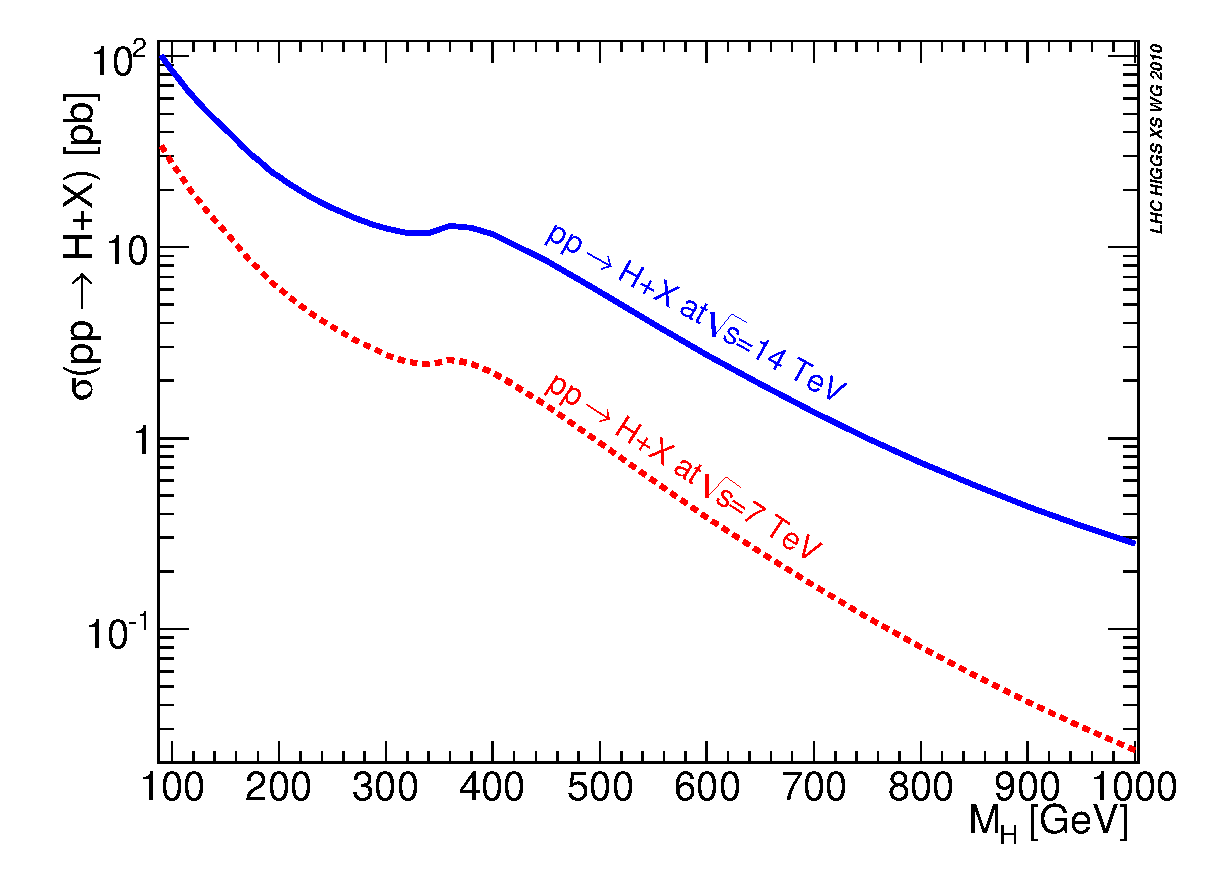
\includegraphics[width=0.8\textwidth]{YRHXS_Summary/YRHXS_Summary_fig1.eps}
	\caption{The total SM Higgs production cross section at
	$\sqrt{s} = 7$\UTeV and $14$\UTeV.}
	\label{fig:totalXS}
	\end{center}
\end{figure}

%-- SM Higgs XS at 7 TeV
\begin{figure}[p]
	\begin{center}
	\includegraphics[width=0.8\textwidth]{YRHXS_Summary/YRHXS_Summary_fig2.eps}
	\caption{The SM Higgs production cross section at $\sqrt{s} = 7$\UTeV.}
	\label{fig:SMXS7TeV}
	\end{center}
\end{figure}

%-- SM Higgs XS at 14 TeV
\begin{figure}[p]
	\begin{center}
	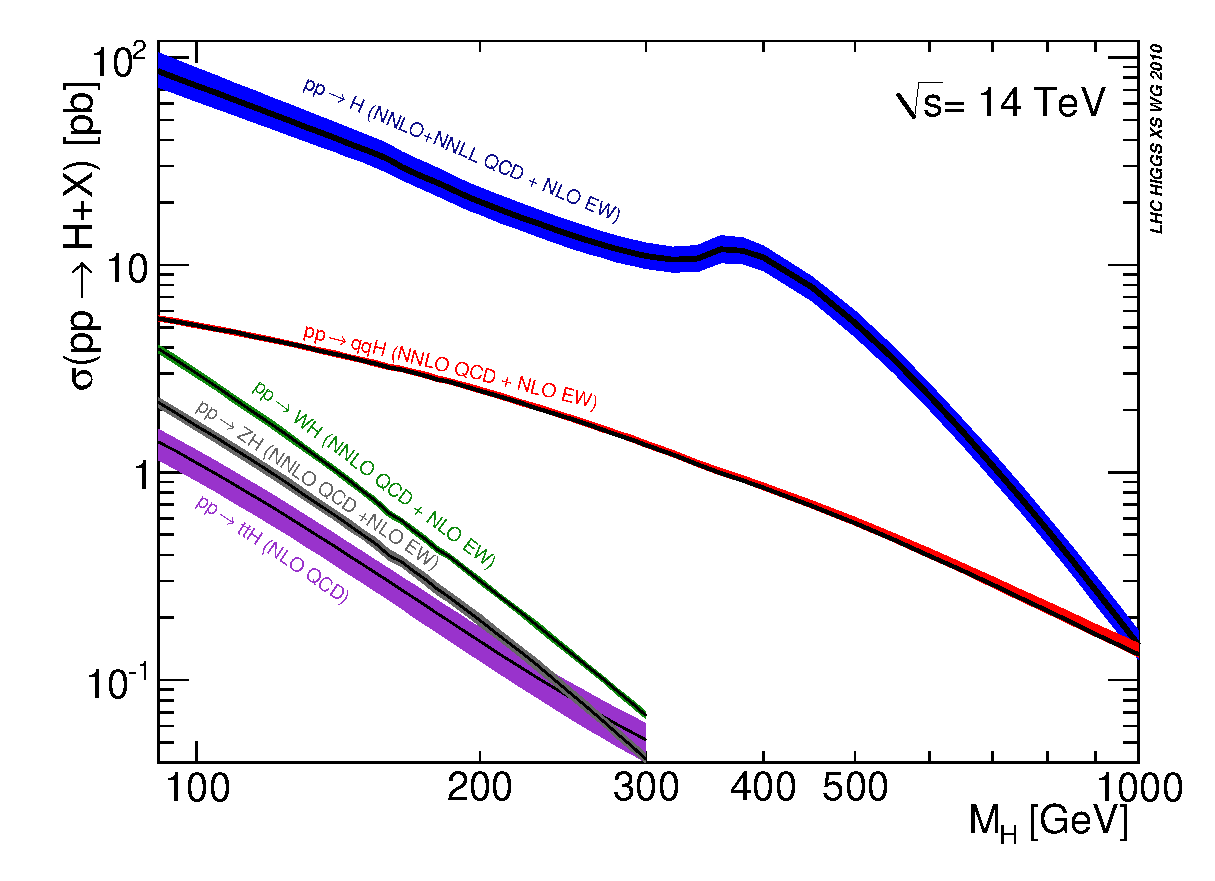
\includegraphics[width=0.8\textwidth]{YRHXS_Summary/YRHXS_Summary_fig3.eps}
	\caption{The SM Higgs production cross section at $\sqrt{s} = 14$\UTeV.}
	\label{fig:SMXS14TeV}
	\end{center}
\end{figure}

%-- SM Higgs BRs
\begin{figure}[!h]
	\begin{center}
	\includegraphics[width=0.8\textwidth]{YRHXS_BR/YRHXS_BR_fig3.eps}
	\caption{The SM Higgs branching ratios as a function of the Higgs-boson
              mass.}
	\label{fig:SMBRs}
	\end{center}
\end{figure}

The combined numbers in this Summary, for the $\Pg\Pg$-fusion process,
are based on the two predictions (ABPS and dFG) of Section~2; work is in
progress to understand the numerical impact of (possibly) remaining THUs with
the inclusion of other analyses (e.g.\ the BD calculation of Section~2.4).

The total cross section at $\sqrt{s} = 7\UTeV$ and $14\UTeV$ is shown in Fig.~\ref{fig:totalXS}.
The SM Higgs production cross sections for the individual channels are shown in
Fig.~\ref{fig:SMXS7TeV} %or Fig.~\ref{fig:SMXS7TeVbw}
for  $\sqrt{s} = 7$\UTeV\ and in
Fig.~\ref{fig:SMXS14TeV} %or Fig.~\ref{fig:SMXS14TeVbw}
for  $\sqrt{s} = 14$\UTeV, with the combined parametric and theoretical uncertainties,
PU + THU, illustrated by bands. 
The labels on the bands briefly indicated the type of radiative corrections that are
included in the predictions.
For details of the calculations and individual components of the error 
(THU, PDF + $\alphas$, etc.) we refer the reader to the main text, e.g.\
to \Sref{ggFsection} for the $\Pg\Pg$-fusion results.
In \Trefs{tab:XS7a}--\ref{tab:XS14b} the cross sections and associated
total errors for different production channels are summarized
together with the total inclusive Higgs production cross sections. 

The branching ratios for the SM Higgs boson are shown in Fig.~\ref{fig:SMBRs}.
Tables containing explicit numbers on partial widths, branching ratios, and on the 
total width can be found in \Sref{sec:BR} and Appendix~\ref{brappendix}.
As already pointed out in \Sref{sec:BR}, a full error analysis of the Higgs branching
ratio is still in progress (see \Bref{Baglio:2010ae} for a recent
independent analysis).

The results shown in this section will be regularly updated at our
webpage\footnote{\sl https://twiki.cern.ch/twiki/bin/view/LHCPhysics/CrossSections}.

Each experiment is recommended to use the common Standard Model input
parameters (\refA{sminput}),
the best known NNLO(NLO) cross sections and branching ratios
reported in this Report as common basis for Higgs physics at LHC.



%-- Perspectives

Beyond the goals of this Report remains the agreement between NLO MC
predictions and NNLO calculations within the acceptance of the detectors.
The next step in the activities of this working group will be the
computation of cross sections that include acceptance cuts and differential
distributions for all final states that will be considered in the Higgs
search at the LHC.
Preferably this should be carried out with the same set of (benchmark) cuts
for ATLAS and CMS.
The goal is to understand how the $K$-factors from (N)LO to (N)NLO will
change after introduction of cuts and to compare the NNLO differential
distributions with the ones from Monte Carlo generators at NLO.

There is a final comment concerning the SM background: We plan to estimate
theoretical predictions for the most important backgrounds in the signal
regions.
This means that a {\em background control region} has to be defined, and
there the experiments will measure a given source of background, directly
from data.
The {\em control region} can be in the bulk of the background production
phase space, but can also be in the tail of the distributions.
Thus it is important to define the precision with which the SM background
will be measured and the theoretical precision available for that particular
region.
Then the background uncertainty should be extrapolated back to the
{\em signal region}, using available theoretical predictions and their
uncertainty.
It will be important to compute the interference between signal and background
and try to access this at NLO.
The (N)LO Monte Carlos will be used to simulate this background and
determine how the $K$-factor is changing with the chosen kinematic cuts.

\vfill


%-- XS Summary Tables

% --- 7 TeV Light Higgs

\begin{landscape}
\begin{table}
	\vspace{-\headsep}
	\begin{center}
	\caption{SM Higgs-boson production cross section at
	$\sqrt{s}=7$\UTeV: light Higgs boson.}
    \small
	\begin{tabular}{r|rc|rc|rc|rc|rc|r}
\hline
$\MH$ & \multicolumn{2}{c|}{ggF} & \multicolumn{2}{c|}{VBF} &
\multicolumn{2}{c|}{WH} & \multicolumn{2}{c|}{ZH} &
\multicolumn{2}{c|}{ttH} &  Total \\
$[\UGeVZ]$ & $~~~~\sigma [\UpbZ]$ & error [\%]
	       & $~~~~\sigma [\UpbZ]$ & error [\%]
	       & $~~~~\sigma [\UpbZ]$ & error [\%]
	       & $~~~~\sigma [\UpbZ]$ & error [\%]
	       & $~~~~\sigma [\UpbZ]$ & error [\%]
	       & $~~~~\sigma [\UpbZ]$ \\
\hline
 $  90$ & $  29.47$ & $ +22.9 \; -\!15.6$ & $  1.710$ & $ +2.7 \; -\!2.3$ & $  1.640$ & $ +3.3 \; -\!3.8$ & $ 0.8597$ & $ +3.9 \; -\!4.0$ & $  0.2162$ & $ +12.5 \; -\!18.1$ & $     33.90$ \\ 
 $  95$ & $  26.58$ & $ +21.9 \; -\!15.9$ & $  1.628$ & $ +2.5 \; -\!2.5$ & $  1.392$ & $ +3.3 \; -\!4.1$ & $ 0.7348$ & $ +4.6 \; -\!4.7$ & $  0.1880$ & $ +12.4 \; -\!18.0$ & $     30.52$ \\ 
 $ 100$ & $  24.02$ & $ +21.2 \; -\!15.6$ & $  1.546$ & $ +2.6 \; -\!2.4$ & $  1.186$ & $ +4.0 \; -\!3.9$ & $ 0.6313$ & $ +4.5 \; -\!4.6$ & $  0.1638$ & $ +12.3 \; -\!18.0$ & $     27.55$ \\ 
 $ 105$ & $  21.78$ & $ +20.8 \; -\!15.5$ & $  1.472$ & $ +2.5 \; -\!2.4$ & $  1.018$ & $ +3.8 \; -\!4.3$ & $ 0.5449$ & $ +5.0 \; -\!5.3$ & $  0.1433$ & $ +12.1 \; -\!17.9$ & $     24.96$ \\ 
 $ 110$ & $  19.84$ & $ +20.4 \; -\!15.3$ & $  1.398$ & $ +2.8 \; -\!2.3$ & $ 0.8754$ & $ +4.1 \; -\!4.5$ & $ 0.4721$ & $ +5.3 \; -\!5.3$ & $  0.1257$ & $ +12.1 \; -\!18.0$ & $     22.71$ \\ 
 $ 115$ & $  18.13$ & $ +20.0 \; -\!15.3$ & $  1.332$ & $ +2.5 \; -\!2.3$ & $ 0.7546$ & $ +4.3 \; -\!4.7$ & $ 0.4107$ & $ +5.5 \; -\!5.4$ & $  0.1106$ & $ +11.9 \; -\!17.8$ & $     20.74$ \\ 
 $ 120$ & $  16.63$ & $ +19.7 \; -\!15.1$ & $  1.269$ & $ +2.8 \; -\!2.5$ & $ 0.6561$ & $ +3.8 \; -\!4.1$ & $ 0.3598$ & $ +5.0 \; -\!4.7$ & $ 0.09756$ & $ +11.8 \; -\!17.8$ & $     19.01$ \\ 
 $ 125$ & $  15.31$ & $ +19.5 \; -\!15.1$ & $  1.211$ & $ +2.7 \; -\!2.4$ & $ 0.5729$ & $ +3.7 \; -\!4.3$ & $ 0.3158$ & $ +4.9 \; -\!5.1$ & $ 0.08634$ & $ +11.8 \; -\!17.8$ & $     17.50$ \\ 
 $ 130$ & $  14.12$ & $ +19.2 \; -\!15.1$ & $  1.154$ & $ +2.8 \; -\!2.3$ & $ 0.5008$ & $ +3.8 \; -\!4.3$ & $ 0.2778$ & $ +5.2 \; -\!5.1$ & $ 0.07658$ & $ +11.6 \; -\!17.7$ & $     16.13$ \\ 
 $ 135$ & $  13.08$ & $ +18.9 \; -\!15.0$ & $  1.100$ & $ +3.0 \; -\!2.2$ & $ 0.4390$ & $ +4.1 \; -\!3.8$ & $ 0.2453$ & $ +5.3 \; -\!5.0$ & $ 0.06810$ & $ +11.5 \; -\!17.6$ & $     14.93$ \\ 
 $ 140$ & $  12.13$ & $ +18.8 \; -\!14.9$ & $  1.052$ & $ +2.8 \; -\!2.2$ & $ 0.3857$ & $ +4.0 \; -\!4.0$ & $ 0.2172$ & $ +5.2 \; -\!5.3$ & $ 0.06072$ & $ +11.4 \; -\!17.6$ & $     13.85$ \\ 
 $ 145$ & $  11.27$ & $ +18.7 \; -\!14.9$ & $  1.004$ & $ +3.1 \; -\!2.1$ & $ 0.3406$ & $ +4.0 \; -\!4.6$ & $ 0.1930$ & $ +5.8 \; -\!5.8$ & $ 0.05435$ & $ +11.4 \; -\!17.6$ & $     12.86$ \\ 
 $ 150$ & $  10.50$ & $ +18.7 \; -\!14.9$ & $ 0.9617$ & $ +2.9 \; -\!2.2$ & $ 0.3001$ & $ +3.7 \; -\!4.1$ & $ 0.1713$ & $ +5.4 \; -\!5.2$ & $ 0.04869$ & $ +11.3 \; -\!17.5$ & $     11.98$ \\ 
 $ 155$ & $  9.795$ & $ +18.5 \; -\!15.0$ & $ 0.9180$ & $ +3.1 \; -\!2.1$ & $ 0.2646$ & $ +4.0 \; -\!4.3$ & $ 0.1525$ & $ +5.7 \; -\!5.2$ & $ 0.04374$ & $ +11.4 \; -\!17.7$ & $     11.17$ \\ 
 $ 160$ & $  9.080$ & $ +18.6 \; -\!15.0$ & $ 0.8787$ & $ +2.9 \; -\!2.3$ & $ 0.2291$ & $ +4.3 \; -\!4.5$ & $ 0.1334$ & $ +6.0 \; -\!5.7$ & $ 0.03942$ & $ +11.4 \; -\!17.7$ & $     10.36$ \\ 
 $ 165$ & $  8.319$ & $ +18.1 \; -\!14.7$ & $ 0.8517$ & $ +3.1 \; -\!2.1$ & $ 0.2107$ & $ +4.1 \; -\!4.3$ & $ 0.1233$ & $ +6.2 \; -\!5.8$ & $ 0.03559$ & $ +11.3 \; -\!17.7$ & $     9.540$ \\ 
 $ 170$ & $  7.729$ & $ +17.9 \; -\!14.9$ & $ 0.8173$ & $ +3.1 \; -\!2.2$ & $ 0.1883$ & $ +4.3 \; -\!4.5$ & $ 0.1106$ & $ +6.4 \; -\!6.1$ & $ 0.03219$ & $ +11.3 \; -\!17.6$ & $     8.877$ \\ 
 $ 175$ & $  7.211$ & $ +17.9 \; -\!14.8$ & $ 0.7814$ & $ +3.2 \; -\!2.1$ & $ 0.1689$ & $ +4.1 \; -\!4.9$ & $0.09950$ & $ +6.2 \; -\!6.0$ & $ 0.02918$ & $ +11.2 \; -\!17.6$ & $     8.290$ \\ 
 $ 180$ & $  6.739$ & $ +18.1 \; -\!14.7$ & $ 0.7480$ & $ +3.1 \; -\!2.4$ & $ 0.1521$ & $ +4.1 \; -\!4.1$ & $0.08917$ & $ +6.0 \; -\!5.7$ & $ 0.02652$ & $ +11.2 \; -\!17.6$ & $     7.755$ \\ 
 $ 185$ & $  6.295$ & $ +17.4 \; -\!15.0$ & $ 0.7193$ & $ +3.4 \; -\!2.2$ & $ 0.1387$ & $ +3.9 \; -\!4.4$ & $0.08139$ & $ +6.1 \; -\!5.8$ & $ 0.02414$ & $ +11.3 \; -\!17.7$ & $     7.259$ \\ 
 $ 190$ & $  5.896$ & $ +17.3 \; -\!15.0$ & $ 0.6925$ & $ +3.3 \; -\!2.2$ & $ 0.1253$ & $ +4.2 \; -\!4.4$ & $0.07366$ & $ +6.1 \; -\!6.0$ & $ 0.02206$ & $ +11.3 \; -\!17.7$ & $     6.810$ \\ 
 $ 195$ & $  5.551$ & $ +17.2 \; -\!15.1$ & $ 0.6643$ & $ +3.4 \; -\!2.5$ & $ 0.1138$ & $ +4.4 \; -\!4.3$ & $0.06699$ & $ +6.3 \; -\!5.9$ & $ 0.02016$ & $ +11.3 \; -\!17.7$ & $     6.416$ \\ 
 $ 200$ & $  5.249$ & $ +17.2 \; -\!15.2$ & $ 0.6371$ & $ +3.4 \; -\!2.3$ & $ 0.1032$ & $ +4.2 \; -\!4.8$ & $0.06096$ & $ +6.4 \; -\!6.0$ & $ 0.01849$ & $ +11.3 \; -\!17.8$ & $     6.069$ \\ 
 $ 210$ & $  4.723$ & $ +16.9 \; -\!15.3$ & $ 0.5869$ & $ +3.5 \; -\!2.4$ & $0.08557$ & $ +4.2 \; -\!4.4$ & $0.05068$ & $ +6.3 \; -\!6.2$ & $ 0.01562$ & $ +11.7 \; -\!18.1$ & $     5.462$ \\ 
 $ 220$ & $  4.288$ & $ +16.8 \; -\!15.3$ & $ 0.5420$ & $ +3.5 \; -\!2.5$ & $0.07142$ & $ +4.0 \; -\!4.6$ & $0.04235$ & $ +6.4 \; -\!6.1$ & $ 0.01330$ & $ +11.8 \; -\!18.2$ & $     4.957$ \\ 
 $ 230$ & $  3.908$ & $ +16.6 \; -\!15.5$ & $ 0.5011$ & $ +3.8 \; -\!2.4$ & $0.06006$ & $ +5.2 \; -\!5.2$ & $0.03560$ & $ +6.9 \; -\!6.7$ & $ 0.01143$ & $ +12.2 \; -\!18.4$ & $     4.516$ \\ 
 $ 240$ & $  3.581$ & $ +16.7 \; -\!15.4$ & $ 0.4641$ & $ +3.8 \; -\!2.5$ & $0.05075$ & $ +4.5 \; -\!4.7$ & $0.02999$ & $ +6.3 \; -\!6.2$ & $0.009873$ & $ +12.3 \; -\!18.6$ & $     4.136$ \\ 
 $ 250$ & $  3.312$ & $ +16.5 \; -\!15.6$ & $ 0.4304$ & $ +4.0 \; -\!2.6$ & $0.04308$ & $ +4.5 \; -\!4.7$ & $0.02540$ & $ +6.2 \; -\!5.8$ & $0.008593$ & $ +12.6 \; -\!18.8$ & $     3.819$ \\ 
 $ 260$ & $  3.072$ & $ +16.2 \; -\!15.9$ & $ 0.3988$ & $ +4.3 \; -\!2.4$ & $0.03674$ & $ +4.8 \; -\!4.7$ & $0.02158$ & $ +6.3 \; -\!6.2$ & $0.007524$ & $ +12.9 \; -\!18.9$ & $     3.537$ \\ 
 $ 270$ & $  2.864$ & $ +16.2 \; -\!15.8$ & $ 0.3715$ & $ +4.2 \; -\!2.6$ & $0.03146$ & $ +4.4 \; -\!4.7$ & $0.01839$ & $ +6.0 \; -\!6.0$ & $0.006636$ & $ +13.6 \; -\!19.4$ & $     3.292$ \\ 
 $ 280$ & $  2.696$ & $ +16.0 \; -\!16.2$ & $ 0.3461$ & $ +4.3 \; -\!2.7$ & $0.02700$ & $ +4.8 \; -\!5.4$ & $0.01575$ & $ +6.5 \; -\!6.2$ & $0.005889$ & $ +14.2 \; -\!19.9$ & $     3.091$ \\ 
 $ 290$ & $  2.546$ & $ +16.1 \; -\!16.1$ & $ 0.3226$ & $ +4.5 \; -\!2.6$ & $0.02333$ & $ +4.9 \; -\!5.0$ & $0.01355$ & $ +6.0 \; -\!5.8$ & $0.005256$ & $ +14.9 \; -\!20.3$ & $     2.911$ \\ 
 $ 300$ & $  2.418$ & $ +16.1 \; -\!16.1$ & $ 0.3010$ & $ +4.6 \; -\!2.7$ & $0.02018$ & $ +5.1 \; -\!5.4$ & $0.01169$ & $ +6.4 \; -\!6.2$ & $0.004719$ & $ +15.6 \; -\!20.9$ & $     2.756$ \\ 
\hline
	\end{tabular}
	\label{tab:XS7a}
	\end{center}
\end{table}
\end{landscape}

% --- 7 TeV Heavy Higgs

\begin{landscape}
\begin{table}
  \begin{center}
	\caption{SM Higgs-boson production cross section at 
	$\sqrt{s}=7$\UTeV: heavy Higgs boson.}    
    \small
	\begin{tabular}{r|rc|rc|r}
\hline
$\MH$ & \multicolumn{2}{c|}{ggF} & \multicolumn{2}{c|}{VBF} &  Total \\
$[\UGeVZ]$ & $~~~~\sigma [\UpbZ]$  & error [\%]
	       & $~~~~\sigma [\UpbZ]$  & error [\%]
	       & $~~~~\sigma [\UpbZ]$ \\
\hline
 $ 320$ & $  2.248$ & $ +16.3 \; -\!16.2$ & $ 0.2622$ & $ +4.9  \; -\!2.7$ &  $     2.510$ \\ 
 $ 340$ & $  2.199$ & $ +17.6 \; -\!15.7$ & $ 0.2286$ & $ +5.1  \; -\!2.9$ &  $     2.428$ \\ 
 $ 360$ & $  2.359$ & $ +19.1 \; -\!14.8$ & $ 0.2018$ & $ +5.3  \; -\!3.0$ &  $     2.561$ \\ 
 $ 380$ & $  2.263$ & $ +16.9 \; -\!15.8$ & $ 0.1807$ & $ +5.7  \; -\!3.0$ &  $     2.444$ \\ 
 $ 400$ & $  2.035$ & $ +15.3 \; -\!16.6$ & $ 0.1619$ & $ +5.9  \; -\!3.0$ &  $     2.197$ \\ 
 $ 450$ & $  1.356$ & $ +16.4 \; -\!17.4$ & $ 0.1235$ & $ +6.6  \; -\!3.2$ &  $     1.479$ \\ 
 $ 500$ & $ 0.8497$ & $ +17.6 \; -\!17.5$ & $0.09491$ & $ +7.2  \; -\!3.4$ &  $    0.9446$ \\ 
 $ 550$ & $ 0.5259$ & $ +18.4 \; -\!17.6$ & $0.07356$ & $ +7.9  \; -\!3.5$ &  $    0.5995$ \\ 
 $ 600$ & $ 0.3275$ & $ +19.3 \; -\!17.8$ & $0.05763$ & $ +8.6  \; -\!3.8$ &  $    0.3851$ \\ 
 $ 650$ & $ 0.2064$ & $ +19.8 \; -\!17.9$ & $0.04556$ & $ +9.3  \; -\!3.8$ &  $    0.2520$ \\ 
 $ 700$ & $ 0.1320$ & $ +20.5 \; -\!18.2$ & $0.03635$ & $ +9.9  \; -\!4.0$ &  $    0.1683$ \\ 
 $ 750$ & $0.08587$ & $ +21.4 \; -\!18.5$ & $0.02924$ & $ +10.7 \; -\!4.2$ &  $    0.1151$ \\ 
 $ 800$ & $0.05665$ & $ +22.1 \; -\!19.0$ & $0.02371$ & $ +11.3 \; -\!4.3$ &  $   0.08036$ \\ 
 $ 850$ & $0.03786$ & $ +23.1 \; -\!19.6$ & $0.01937$ & $ +11.9 \; -\!4.5$ &  $   0.05723$ \\ 
 $ 900$ & $0.02561$ & $ +24.3 \; -\!20.4$ & $0.01595$ & $ +12.6 \; -\!4.6$ &  $   0.04156$ \\ 
 $ 950$ & $0.01752$ & $ +25.5 \; -\!21.4$ & $0.01321$ & $ +13.4 \; -\!4.8$ &  $   0.03073$ \\ 
 $1000$ & $0.01210$ & $ +27.1 \; -\!22.6$ & $0.01103$ & $ +14.2 \; -\!4.9$ &  $   0.02313$ \\ 
\hline
	\end{tabular}
	\label{tab:XS7b}
	\end{center}
\end{table}
\end{landscape}


% --- 14 TeV Light Higgs

\begin{landscape}
\begin{table}
	\vspace{-\headsep}
	\begin{center}
	\caption{SM Higgs-boson production cross section at 
	$\sqrt{s}=14$\UTeV: light Higgs boson.}
    \small
	\begin{tabular}{r|rc|rc|rc|rc|rc|r}
\hline
$\MH$ & \multicolumn{2}{c|}{ggF} & \multicolumn{2}{c|}{VBF} &
\multicolumn{2}{c|}{WH} & \multicolumn{2}{c|}{ZH} &
\multicolumn{2}{c|}{ttH} &  Total \\
$[\UGeVZ]$ & $~~~~\sigma [\UpbZ]$ & error [\%]
	       & $~~~~\sigma [\UpbZ]$ & error [\%]
	       & $~~~~\sigma [\UpbZ]$ & error [\%]
	       & $~~~~\sigma [\UpbZ]$ & error [\%]
	       & $~~~~\sigma [\UpbZ]$ & error [\%]
	       & $~~~~\sigma [\UpbZ]$ \\
\hline
 $  90$ & $  87.55$ & $ +23.0 \; -\!16.4$ & $  5.569$ & $ +2.9 \; -\!3.0$ & $  4.090$ & $ +4.3 \; -\!4.6$ & $  2.245$ & $ +5.3 \; -\!5.7$ & $   1.449$ & $ +14.9 \; -\!18.0$ & $     100.9$ \\ 
 $  95$ & $  79.83$ & $ +22.3 \; -\!16.0$ & $  5.338$ & $ +3.0 \; -\!3.1$ & $  3.499$ & $ +4.4 \; -\!4.5$ & $  1.941$ & $ +5.2 \; -\!5.2$ & $   1.268$ & $ +14.8 \; -\!18.0$ & $     91.88$ \\ 
 $ 100$ & $  73.27$ & $ +21.5 \; -\!16.0$ & $  5.114$ & $ +2.8 \; -\!3.1$ & $  3.002$ & $ +4.5 \; -\!4.3$ & $  1.683$ & $ +5.7 \; -\!5.3$ & $   1.114$ & $ +14.8 \; -\!18.0$ & $     84.18$ \\ 
 $ 105$ & $  67.34$ & $ +21.1 \; -\!15.6$ & $  4.900$ & $ +3.2 \; -\!2.9$ & $  2.596$ & $ +4.1 \; -\!4.0$ & $  1.468$ & $ +5.4 \; -\!5.4$ & $  0.9816$ & $ +14.7 \; -\!18.0$ & $     77.29$ \\ 
 $ 110$ & $  62.16$ & $ +20.6 \; -\!15.3$ & $  4.750$ & $ +2.2 \; -\!3.9$ & $  2.246$ & $ +4.1 \; -\!4.6$ & $  1.283$ & $ +6.1 \; -\!5.6$ & $  0.8681$ & $ +14.8 \; -\!18.1$ & $     71.31$ \\ 
 $ 115$ & $  57.57$ & $ +20.2 \; -\!15.0$ & $  4.520$ & $ +2.9 \; -\!3.0$ & $  1.952$ & $ +4.5 \; -\!4.0$ & $  1.130$ & $ +6.2 \; -\!5.2$ & $  0.7699$ & $ +14.8 \; -\!18.1$ & $     65.94$ \\ 
 $ 120$ & $  53.49$ & $ +20.0 \; -\!14.8$ & $  4.361$ & $ +2.5 \; -\!3.5$ & $  1.710$ & $ +4.4 \; -\!4.1$ & $ 0.9967$ & $ +6.0 \; -\!5.4$ & $  0.6850$ & $ +14.7 \; -\!18.1$ & $     61.24$ \\ 
 $ 125$ & $  49.85$ & $ +19.6 \; -\!14.6$ & $  4.180$ & $ +2.8 \; -\!3.0$ & $  1.504$ & $ +4.1 \; -\!4.4$ & $ 0.8830$ & $ +6.4 \; -\!5.5$ & $  0.6113$ & $ +14.8 \; -\!18.2$ & $     57.03$ \\ 
 $ 130$ & $  46.55$ & $ +19.5 \; -\!14.4$ & $  4.029$ & $ +2.5 \; -\!3.1$ & $  1.324$ & $ +3.8 \; -\!3.7$ & $ 0.7846$ & $ +6.3 \; -\!5.2$ & $  0.5472$ & $ +14.8 \; -\!18.2$ & $     53.23$ \\ 
 $ 135$ & $  43.61$ & $ +19.1 \; -\!14.2$ & $  3.862$ & $ +3.1 \; -\!2.8$ & $  1.167$ & $ +3.5 \; -\!3.4$ & $ 0.6981$ & $ +5.9 \; -\!5.2$ & $  0.4910$ & $ +14.8 \; -\!18.2$ & $     49.83$ \\ 
 $ 140$ & $  40.93$ & $ +18.9 \; -\!13.9$ & $  3.732$ & $ +2.6 \; -\!3.3$ & $  1.034$ & $ +3.3 \; -\!3.8$ & $ 0.6256$ & $ +5.8 \; -\!5.2$ & $  0.4419$ & $ +14.8 \; -\!18.2$ & $     46.76$ \\ 
 $ 145$ & $  38.49$ & $ +18.8 \; -\!13.7$ & $  3.590$ & $ +3.0 \; -\!3.0$ & $ 0.9200$ & $ +3.8 \; -\!3.7$ & $ 0.5601$ & $ +6.7 \; -\!5.5$ & $  0.3989$ & $ +14.9 \; -\!18.3$ & $     43.96$ \\ 
 $ 150$ & $  36.27$ & $ +18.7 \; -\!13.5$ & $  3.460$ & $ +2.8 \; -\!3.0$ & $ 0.8156$ & $ +3.0 \; -\!3.3$ & $ 0.5016$ & $ +6.0 \; -\!4.7$ & $  0.3609$ & $ +14.9 \; -\!18.3$ & $     41.41$ \\ 
 $ 155$ & $  34.22$ & $ +18.6 \; -\!13.6$ & $  3.332$ & $ +2.9 \; -\!3.0$ & $ 0.7255$ & $ +3.5 \; -\!3.7$ & $ 0.4513$ & $ +6.5 \; -\!5.6$ & $  0.3275$ & $ +14.9 \; -\!18.4$ & $     39.06$ \\ 
 $ 160$ & $  32.10$ & $ +18.6 \; -\!13.7$ & $  3.198$ & $ +3.1 \; -\!2.8$ & $ 0.6341$ & $ +3.3 \; -\!3.6$ & $ 0.3986$ & $ +6.6 \; -\!5.5$ & $  0.2980$ & $ +15.0 \; -\!18.5$ & $     36.63$ \\ 
 $ 165$ & $  29.77$ & $ +17.8 \; -\!13.4$ & $  3.137$ & $ +3.0 \; -\!2.9$ & $ 0.5850$ & $ +2.6 \; -\!3.0$ & $ 0.3705$ & $ +6.4 \; -\!4.9$ & $  0.2718$ & $ +15.1 \; -\!18.5$ & $     34.13$ \\ 
 $ 170$ & $  27.93$ & $ +17.7 \; -\!13.3$ & $  3.033$ & $ +2.8 \; -\!3.0$ & $ 0.5260$ & $ +3.1 \; -\!3.5$ & $ 0.3355$ & $ +6.5 \; -\!5.4$ & $  0.2487$ & $ +15.7 \; -\!18.9$ & $     32.07$ \\ 
 $ 175$ & $  26.36$ & $ +17.7 \; -\!13.4$ & $  2.922$ & $ +3.5 \; -\!2.8$ & $ 0.4763$ & $ +3.4 \; -\!3.2$ & $ 0.3044$ & $ +6.6 \; -\!5.7$ & $  0.2279$ & $ +15.8 \; -\!18.9$ & $     30.29$ \\ 
 $ 180$ & $  24.92$ & $ +17.8 \; -\!13.4$ & $  2.805$ & $ +3.3 \; -\!2.8$ & $ 0.4274$ & $ +3.2 \; -\!3.4$ & $ 0.2744$ & $ +6.7 \; -\!5.8$ & $  0.2095$ & $ +15.8 \; -\!19.0$ & $     28.64$ \\ 
 $ 185$ & $  23.49$ & $ +17.2 \; -\!13.4$ & $  2.740$ & $ +2.8 \; -\!2.9$ & $ 0.3963$ & $ +2.9 \; -\!3.2$ & $ 0.2524$ & $ +6.1 \; -\!5.5$ & $  0.1930$ & $ +15.8 \; -\!19.0$ & $     27.07$ \\ 
 $ 190$ & $  22.21$ & $ +17.1 \; -\!13.2$ & $  2.652$ & $ +2.7 \; -\!2.9$ & $ 0.3600$ & $ +3.0 \; -\!3.4$ & $ 0.2301$ & $ +6.5 \; -\!5.9$ & $  0.1783$ & $ +16.0 \; -\!19.2$ & $     25.63$ \\ 
 $ 195$ & $  21.10$ & $ +17.0 \; -\!13.2$ & $  2.566$ & $ +2.9 \; -\!2.9$ & $ 0.3291$ & $ +3.0 \; -\!3.4$ & $ 0.2112$ & $ +6.4 \; -\!5.8$ & $  0.1650$ & $ +16.0 \; -\!19.2$ & $     24.37$ \\ 
 $ 200$ & $  20.16$ & $ +16.8 \; -\!13.2$ & $  2.472$ & $ +3.2 \; -\!2.7$ & $ 0.3004$ & $ +3.4 \; -\!3.5$ & $ 0.1936$ & $ +6.7 \; -\!6.1$ & $  0.1532$ & $ +16.2 \; -\!19.4$ & $     23.28$ \\ 
 $ 210$ & $  18.49$ & $ +16.6 \; -\!13.3$ & $  2.315$ & $ +3.2 \; -\!2.7$ & $ 0.2526$ & $ +2.8 \; -\!3.3$ & $ 0.1628$ & $ +6.5 \; -\!5.1$ & $  0.1329$ & $ +16.4 \; -\!19.5$ & $     21.35$ \\ 
 $ 220$ & $  17.08$ & $ +16.4 \; -\!13.3$ & $  2.171$ & $ +2.9 \; -\!3.1$ & $ 0.2138$ & $ +3.4 \; -\!3.3$ & $ 0.1380$ & $ +6.3 \; -\!5.6$ & $  0.1162$ & $ +16.7 \; -\!19.8$ & $     19.72$ \\ 
 $ 230$ & $  15.86$ & $ +16.3 \; -\!13.2$ & $  2.036$ & $ +3.2 \; -\!2.8$ & $ 0.1826$ & $ +3.9 \; -\!4.0$ & $ 0.1173$ & $ +7.0 \; -\!6.2$ & $  0.1025$ & $ +17.1 \; -\!20.0$ & $     18.30$ \\ 
 $ 240$ & $  14.82$ & $ +16.1 \; -\!13.2$ & $  1.918$ & $ +3.0 \; -\!2.7$ & $ 0.1561$ & $ +3.7 \; -\!3.8$ & $0.09996$ & $ +6.5 \; -\!5.9$ & $ 0.09109$ & $ +17.3 \; -\!20.3$ & $     17.09$ \\ 
 $ 250$ & $  13.92$ & $ +16.0 \; -\!13.2$ & $  1.807$ & $ +2.9 \; -\!3.0$ & $ 0.1343$ & $ +3.2 \; -\!3.7$ & $0.08540$ & $ +6.2 \; -\!5.5$ & $ 0.08156$ & $ +17.7 \; -\!20.5$ & $     16.03$ \\ 
 $ 260$ & $  13.14$ & $ +15.9 \; -\!13.3$ & $  1.711$ & $ +2.9 \; -\!3.7$ & $ 0.1161$ & $ +3.0 \; -\!3.5$ & $0.07341$ & $ +6.1 \; -\!5.2$ & $ 0.07351$ & $ +18.1 \; -\!20.8$ & $     15.11$ \\ 
 $ 270$ & $  12.47$ & $ +15.7 \; -\!13.1$ & $  1.606$ & $ +3.0 \; -\!2.9$ & $ 0.1009$ & $ +3.1 \; -\!3.2$ & $0.06325$ & $ +5.3 \; -\!4.7$ & $ 0.06667$ & $ +18.5 \; -\!21.1$ & $     14.31$ \\ 
 $ 280$ & $  11.90$ & $ +15.7 \; -\!13.1$ & $  1.514$ & $ +3.2 \; -\!2.7$ & $0.08781$ & $ +3.4 \; -\!3.6$ & $0.05474$ & $ +5.7 \; -\!5.0$ & $ 0.06081$ & $ +19.0 \; -\!21.4$ & $     13.62$ \\ 
 $ 290$ & $  11.43$ & $ +15.4 \; -\!13.2$ & $  1.436$ & $ +3.2 \; -\!2.8$ & $0.07714$ & $ +3.5 \; -\!3.8$ & $0.04769$ & $ +5.4 \; -\!4.7$ & $ 0.05575$ & $ +19.4 \; -\!21.7$ & $     13.05$ \\ 
 $ 300$ & $  11.05$ & $ +15.3 \; -\!13.0$ & $  1.358$ & $ +3.2 \; -\!2.9$ & $0.06755$ & $ +3.9 \; -\!3.8$ & $0.04156$ & $ +5.6 \; -\!5.2$ & $ 0.05133$ & $ +19.8 \; -\!21.9$ & $     12.57$ \\ 
\hline
	\end{tabular}
	\label{tab:XS14a}
	\end{center}
\end{table}
\end{landscape}

% --- 14 TeV Heavy Higgs

\begin{landscape}
\begin{table}
  \begin{center}
	\caption{SM Higgs-boson production cross section at 
	$\sqrt{s}=14$\UTeV: heavy Higgs boson.}    
    \small
	\begin{tabular}{r|rc|rc|r}
\hline
$\MH$ & \multicolumn{2}{c|}{ggF} & \multicolumn{2}{c|}{VBF} &  Total \\
$[\UGeVZ]$ & $~~~~\sigma [\UpbZ]$  & error [\%]
	       & $~~~~\sigma [\UpbZ]$  & error [\%]
	       & $~~~~\sigma [\UpbZ]$ \\
\hline
 $ 320$ & $  10.59$ & $ +15.4 \; -\!12.9$ & $  1.220$ & $ +3.2 \; -\!2.8$   & $      11.81$ \\ 
 $ 340$ & $  10.72$ & $ +15.9 \; -\!13.4$ & $  1.094$ & $ +3.3 \; -\!2.8$   & $      11.81$ \\ 
 $ 360$ & $  11.91$ & $ +16.5 \; -\!13.8$ & $ 0.9930$ & $ +3.3 \; -\!2.8$   & $      12.90$ \\ 
 $ 380$ & $  11.72$ & $ +15.3 \; -\!13.3$ & $ 0.9148$ & $ +3.4 \; -\!2.7$   & $      12.63$ \\ 
 $ 400$ & $  10.87$ & $ +13.2 \; -\!13.6$ & $ 0.8422$ & $ +3.6 \; -\!2.7$   & $      11.71$ \\ 
 $ 450$ & $  7.790$ & $ +12.6 \; -\!13.7$ & $ 0.6893$ & $ +3.8 \; -\!3.0$   & $      8.479$ \\ 
 $ 500$ & $  5.255$ & $ +13.7 \; -\!13.9$ & $ 0.5684$ & $ +4.0 \; -\!2.9$   & $      5.823$ \\ 
 $ 550$ & $  3.493$ & $ +14.2 \; -\!14.1$ & $ 0.4724$ & $ +4.4 \; -\!3.0$   & $      3.965$ \\ 
 $ 600$ & $  2.332$ & $ +14.5 \; -\!14.0$ & $ 0.3965$ & $ +4.7 \; -\!3.1$   & $      2.728$ \\ 
 $ 650$ & $  1.576$ & $ +14.5 \; -\!13.8$ & $ 0.3360$ & $ +4.9 \; -\!3.2$   & $      1.912$ \\ 
 $ 700$ & $  1.078$ & $ +15.2 \; -\!14.1$ & $ 0.2872$ & $ +5.2 \; -\!3.4$   & $      1.365$ \\ 
 $ 750$ & $ 0.7498$ & $ +15.5 \; -\!13.9$ & $ 0.2476$ & $ +5.6 \; -\!3.5$   & $     0.9974$ \\ 
 $ 800$ & $ 0.5280$ & $ +15.6 \; -\!14.0$ & $ 0.2155$ & $ +5.8 \; -\!3.7$   & $     0.7435$ \\ 
 $ 850$ & $ 0.3766$ & $ +15.9 \; -\!14.2$ & $ 0.1885$ & $ +6.3 \; -\!3.6$   & $     0.5651$ \\ 
 $ 900$ & $ 0.2723$ & $ +16.3 \; -\!14.5$ & $ 0.1666$ & $ +6.5 \; -\!3.8$   & $     0.4389$ \\ 
 $ 950$ & $ 0.1987$ & $ +16.8 \; -\!14.5$ & $ 0.1484$ & $ +6.6 \; -\!4.0$   & $     0.3471$ \\ 
 $1000$ & $ 0.1472$ & $ +16.8 \; -\!14.6$ & $ 0.1330$ & $ +7.0 \; -\!4.0$   & $     0.2802$ \\ 
\hline
	\end{tabular}
	\label{tab:XS14b}
	\end{center}
\end{table}
\end{landscape}
